%==============================================================================00
% Options for packages loaded elsewhere
\PassOptionsToPackage{unicode}{hyperref}
\PassOptionsToPackage{hyphens}{url}
%==============================================================================01
\documentclass[11pt, oneside, openany]{scrbook}
\setkomafont{disposition}{\bfseries}
\usepackage{mathptmx}
\usepackage{lipsum}
%==============================================================================02
% Make chapter pages have numbering at top right
\usepackage{fancyhdr}
\pagestyle{fancy}
\lhead{}
\chead{}
\rhead{\thepage}
\lfoot{}
\cfoot{}
\rfoot{}
\renewcommand{\headrulewidth}{0pt}
\makeatletter
\renewcommand\chapter{\if@openright\cleardoublepage\else\clearpage\fi
                    \thispagestyle{fancy}%
                    \global\@topnum\z@
                    \@afterindentfalse
                    \secdef\@chapter\@schapter}
\makeatother
%==============================================================================03
\usepackage{lmodern}
\usepackage{setspace}
%==============================================================================04
\usepackage{amssymb,amsmath}
%==============================================================================05
\usepackage{ifxetex,ifluatex}
\ifnum 0\ifxetex 1\fi\ifluatex 1\fi=0 % if pdftex
  \usepackage[T1]{fontenc}
  \usepackage[utf8]{inputenc}
  \usepackage{textcomp} % provide euro and other symbols
\else % if luatex or xetex
  \usepackage{unicode-math}
  \defaultfontfeatures{Scale=MatchLowercase}
  \defaultfontfeatures[\rmfamily]{Ligatures=TeX,Scale=1}
\fi
%==============================================================================06
% Use upquote if available, for straight quotes in verbatim environments
\IfFileExists{upquote.sty}{\usepackage{upquote}}{}
\IfFileExists{microtype.sty}{% use microtype if available
  \usepackage[]{microtype}
  \UseMicrotypeSet[protrusion]{basicmath} % disable protrusion for tt fonts
}{}
\makeatletter
\@ifundefined{KOMAClassName}{% if non-KOMA class
  \IfFileExists{parskip.sty}{%
    \usepackage{parskip}
  }{% else
    \setlength{\parindent}{0pt}
    \setlength{\parskip}{6pt plus 2pt minus 1pt}}
}{% if KOMA class
  \KOMAoptions{parskip=half}}
\makeatother
%==============================================================================07
\usepackage[table]{xcolor}
%==============================================================================08
\IfFileExists{xurl.sty}{\usepackage{xurl}}{} % add URL line breaks if available
\IfFileExists{bookmark.sty}{\usepackage{bookmark}}{\usepackage{hyperref}}
\hypersetup{
  pdftitle={A Tale of Two Cities: Reno and Las Vegas},
  pdfauthor={Karen T. Barensby},
  hidelinks,
  pdfcreator={LaTeX via pandoc}}
\urlstyle{same} % disable monospaced font for URLs
%==============================================================================09
\usepackage[top=1in, left=1.5in, bottom=1.25in, right=1.5in]{geometry}
%==============================================================================10
\usepackage{color}
\usepackage{fancyvrb}
\newcommand{\VerbBar}{|}
\newcommand{\VERB}{\Verb[commandchars=\\\{\}]}
\DefineVerbatimEnvironment{Highlighting}{Verbatim}{commandchars=\\\{\}}
% Add ',fontsize=\small' for more characters per line
\usepackage{framed}
\definecolor{shadecolor}{RGB}{248,248,248}
\newenvironment{Shaded}{\begin{snugshade}}{\end{snugshade}}
\newcommand{\AlertTok}[1]{\textcolor[rgb]{0.94,0.16,0.16}{#1}}
\newcommand{\AnnotationTok}[1]{\textcolor[rgb]{0.56,0.35,0.01}{\textbf{\textit{#1}}}}
\newcommand{\AttributeTok}[1]{\textcolor[rgb]{0.77,0.63,0.00}{#1}}
\newcommand{\BaseNTok}[1]{\textcolor[rgb]{0.00,0.00,0.81}{#1}}
\newcommand{\BuiltInTok}[1]{#1}
\newcommand{\CharTok}[1]{\textcolor[rgb]{0.31,0.60,0.02}{#1}}
\newcommand{\CommentTok}[1]{\textcolor[rgb]{0.56,0.35,0.01}{\textit{#1}}}
\newcommand{\CommentVarTok}[1]{\textcolor[rgb]{0.56,0.35,0.01}{\textbf{\textit{#1}}}}
\newcommand{\ConstantTok}[1]{\textcolor[rgb]{0.00,0.00,0.00}{#1}}
\newcommand{\ControlFlowTok}[1]{\textcolor[rgb]{0.13,0.29,0.53}{\textbf{#1}}}
\newcommand{\DataTypeTok}[1]{\textcolor[rgb]{0.13,0.29,0.53}{#1}}
\newcommand{\DecValTok}[1]{\textcolor[rgb]{0.00,0.00,0.81}{#1}}
\newcommand{\DocumentationTok}[1]{\textcolor[rgb]{0.56,0.35,0.01}{\textbf{\textit{#1}}}}
\newcommand{\ErrorTok}[1]{\textcolor[rgb]{0.64,0.00,0.00}{\textbf{#1}}}
\newcommand{\ExtensionTok}[1]{#1}
\newcommand{\FloatTok}[1]{\textcolor[rgb]{0.00,0.00,0.81}{#1}}
\newcommand{\FunctionTok}[1]{\textcolor[rgb]{0.00,0.00,0.00}{#1}}
\newcommand{\ImportTok}[1]{#1}
\newcommand{\InformationTok}[1]{\textcolor[rgb]{0.56,0.35,0.01}{\textbf{\textit{#1}}}}
\newcommand{\KeywordTok}[1]{\textcolor[rgb]{0.13,0.29,0.53}{\textbf{#1}}}
\newcommand{\NormalTok}[1]{#1}
\newcommand{\OperatorTok}[1]{\textcolor[rgb]{0.81,0.36,0.00}{\textbf{#1}}}
\newcommand{\OtherTok}[1]{\textcolor[rgb]{0.56,0.35,0.01}{#1}}
\newcommand{\PreprocessorTok}[1]{\textcolor[rgb]{0.56,0.35,0.01}{\textit{#1}}}
\newcommand{\RegionMarkerTok}[1]{#1}
\newcommand{\SpecialCharTok}[1]{\textcolor[rgb]{0.00,0.00,0.00}{#1}}
\newcommand{\SpecialStringTok}[1]{\textcolor[rgb]{0.31,0.60,0.02}{#1}}
\newcommand{\StringTok}[1]{\textcolor[rgb]{0.31,0.60,0.02}{#1}}
\newcommand{\VariableTok}[1]{\textcolor[rgb]{0.00,0.00,0.00}{#1}}
\newcommand{\VerbatimStringTok}[1]{\textcolor[rgb]{0.31,0.60,0.02}{#1}}
\newcommand{\WarningTok}[1]{\textcolor[rgb]{0.56,0.35,0.01}{\textbf{\textit{#1}}}}
%==============================================================================11
\usepackage{longtable,booktabs}
% Correct order of tables after \paragraph or \subparagraph
\usepackage{etoolbox}
\makeatletter
\patchcmd\longtable{\par}{\if@noskipsec\mbox{}\fi\par}{}{}
\makeatother
% Allow footnotes in longtable head/foot
\IfFileExists{footnotehyper.sty}{\usepackage{footnotehyper}}{\usepackage{footnote}}
\makesavenoteenv{longtable}
%==============================================================================12
\usepackage{graphicx}
\makeatletter
\def\maxwidth{\ifdim\Gin@nat@width>\linewidth\linewidth\else\Gin@nat@width\fi}
\def\maxheight{\ifdim\Gin@nat@height>\textheight\textheight\else\Gin@nat@height\fi}
\makeatother
% Scale images if necessary, so that they will not overflow the page
% margins by default, and it is still possible to overwrite the defaults
% using explicit options in \includegraphics[width, height, ...]{}
\setkeys{Gin}{width=\maxwidth,height=\maxheight,keepaspectratio}
% Set default figure placement to htbp
\makeatletter
\def\fps@figure{htbp}
\makeatother
%==============================================================================13
%==============================================================================14
%==============================================================================15
\setlength{\emergencystretch}{3em} % prevent overfull lines
\providecommand{\tightlist}{%
  \setlength{\itemsep}{0pt}\setlength{\parskip}{0pt}}
%==============================================================================16
\setcounter{secnumdepth}{5}
%==============================================================================17
%==============================================================================18
% Place here anything extra that you would like in the preamble
%==============================================================================19
\ifluatex
  \usepackage{selnolig}  % disable illegal ligatures
\fi
%==============================================================================20
\usepackage[]{natbib}
\bibliographystyle{apalike}
%==============================================================================21
\frontmatter

\begin{document}

\begin{titlepage}
\begin{center}
\vspace*{1in}
University of Nevada, Reno

\vspace{1.5in}
\textbf{A Tale of Two Cities: Reno and Las Vegas}

\vspace{1in}
A thesis submitted in partial fulfillment of the \\
requirements for the degree of Master of Science in \\
Statistics and Data Science

\vspace{1in}
by

\vspace{1em}
Karen T. Barensby

\vspace{2em}
Dr.~Glen J. Smith/Thesis Advisor

\vspace{3em}
May/August/December, 20XX

\end{center}
\end{titlepage}
%==============================================================================22
% Begin Copyright --------------------- (optional)
\thispagestyle{empty}
\begin{center}
\vspace*{\fill}
Copyright by Albert Einstein 1944 \\
All Rights Reserved
\vspace*{\fill}
\end{center}
%------------------------ End Copyright


% Begin Committee Approval Page -------
\newpage
\thispagestyle{empty}
\begin{center}


\includegraphics[width=0.75in, height=0.75in]{./figures/unr_logos/University Logo RGB_block_n_blue}

THE GRADUATE SCHOOL

\vspace{1em}
We recommend that the thesis \\
prepared under our supervision by\\

\vspace{1em}
\textbf{YOUR NAME}

\vspace{1em}
entitled

\textbf{THESIS TITLE}

\vspace{2em}
be accepted in partial fullfilment of the \\
requirements for the degree of

\vspace{1em}
\textbf{DEGREE}

\vspace{1em}
ADVISOR \\
\textit{Advisor}

\vspace{1em}
COMMITTEE MEMBER \\
\textit{Committee Member}

\vspace{1em}
GRADUATE SCHOOL REPRESENTATIVE \\
\textit{Graduate School Representative}

\vspace{1em}
David W. Zeh, Ph.D., Dean \\
\textit{Graduate School}

\vspace{1em}
May/August/December, 20XX
\end{center}
%---------- End Committee Approval Page


% Begin ---------------
\newpage
\setcounter{page}{1} % Begin lower case Roman numerals
\section*{Abstract}
\lipsum[1]
%------------------ End


% Begin ---------------
\newpage
\section*{Dedication (optional)}
\lipsum[2]
%------------------ End


% Begin ---------------
\newpage
\section*{Acknowledgments (optional)}
\lipsum[1]
%------------------ End

% Begin ---------------
\setcounter{tocdepth}{1}
\tableofcontents

\listoftables

\listoffigures
%------------------ End
%==============================================================================23
\setstretch{2.0}
%==============================================================================24
\mainmatter
%==============================================================================25
\hypertarget{ch1}{%
\chapter{Introduction}\label{ch1}}

example of r plot

\begin{figure}

{\centering 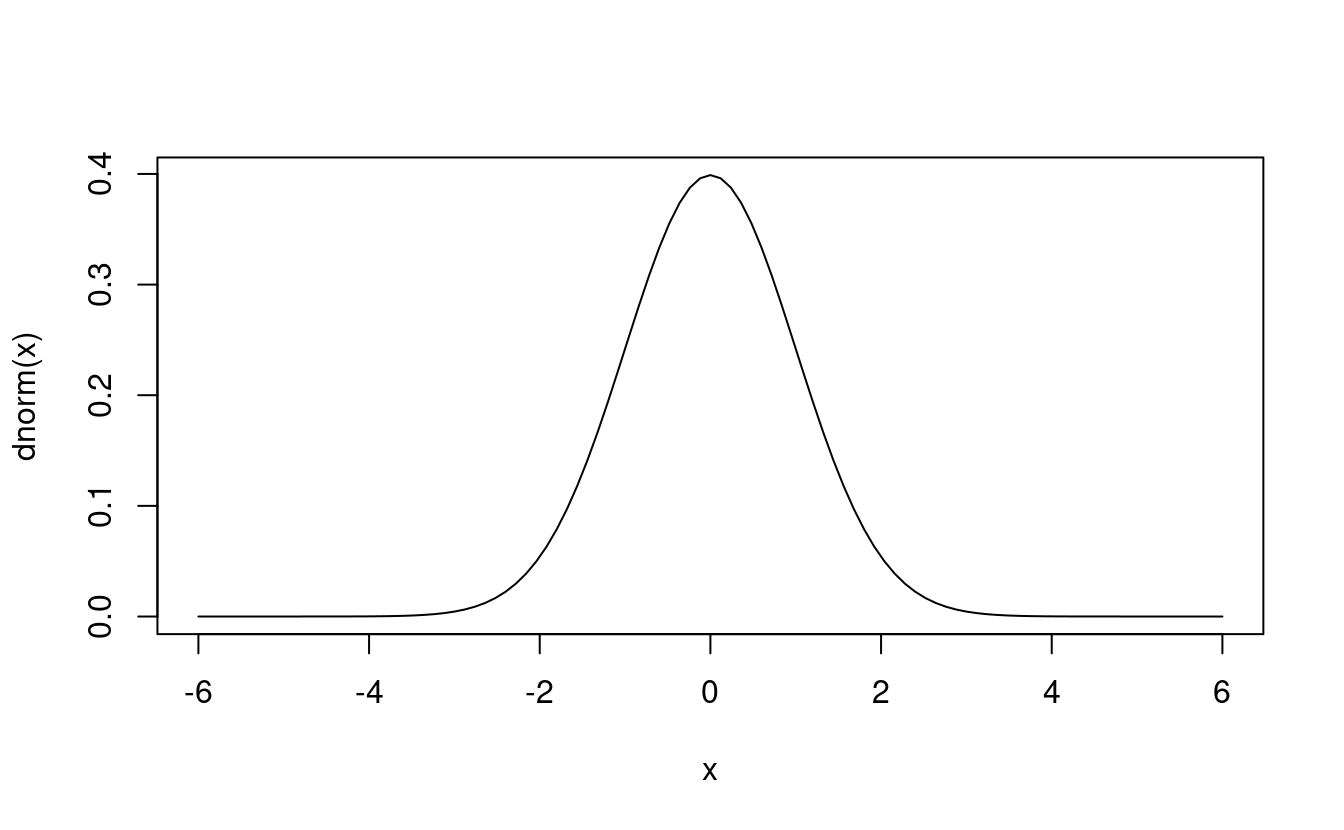
\includegraphics[width=0.7\linewidth]{index_files/figure-latex/rplot-1} 

}

\caption{My first figure}\label{fig:rplot}
\end{figure}

example of ggplot

\begin{figure}

{\centering 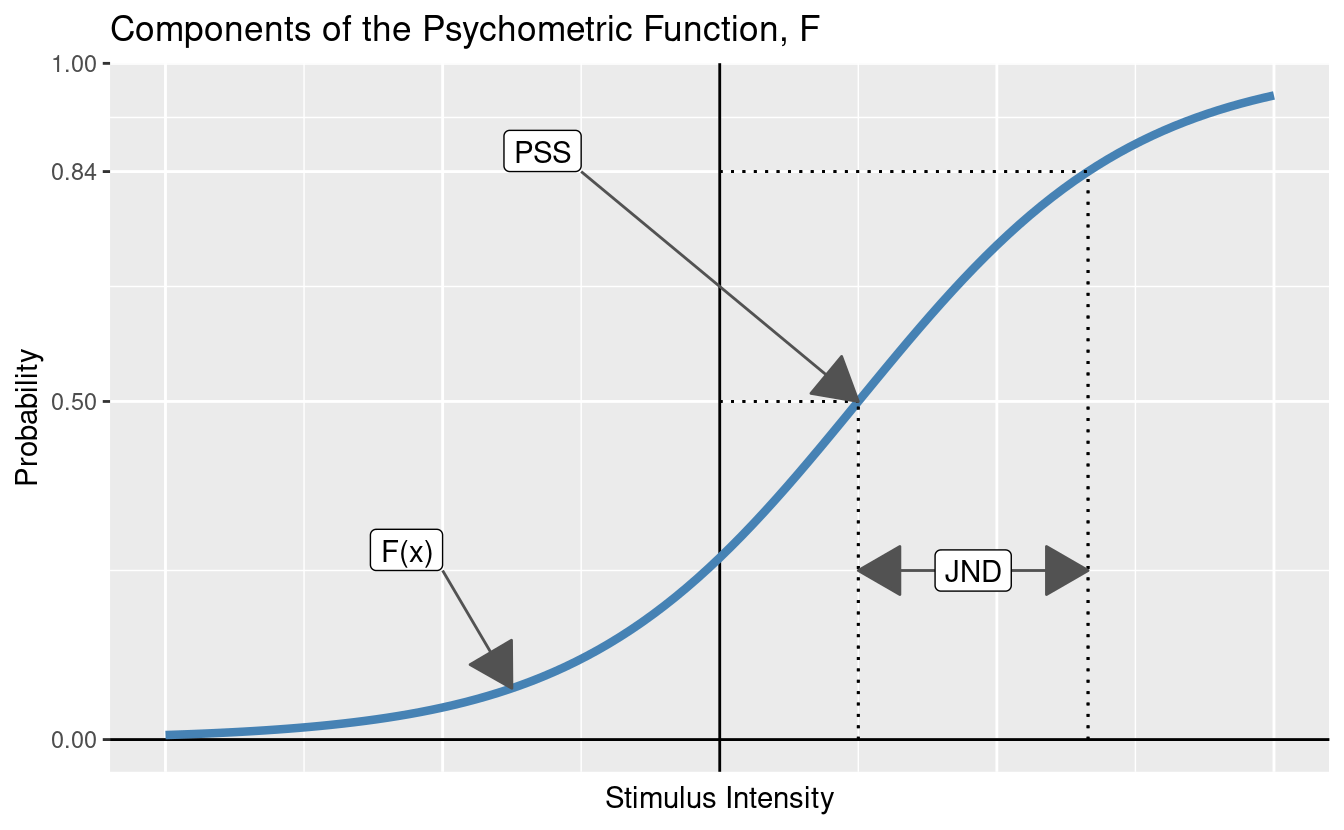
\includegraphics[width=0.7\linewidth]{index_files/figure-latex/ggplot-1} 

}

\caption{My second figure}\label{fig:ggplot}
\end{figure}

example of included graphics

\begin{figure}

{\centering 
\includegraphics[width=0.7\linewidth]{figures/unr_logos/University Logo RGB_block_n_blue_877} 

}

\caption{My third figure}\label{fig:png}
\end{figure}

\hypertarget{ch2}{%
\chapter{Using Tables}\label{ch2}}

example of a reference \citep{britannica2014editors}.

example of display math

\[
\frac{\Delta I}{I} = k
\]

Example of inline math \(\Delta I = 0.2\)

\hypertarget{level-2-heading}{%
\section{Level 2 Heading}\label{level-2-heading}}

example of a table and reference (table \ref{tab:my-table})

\begin{table}[!h]

\caption{\label{tab:my-table}THIS IS MY TABLE!}
\centering
\begin{tabular}[t]{rrrrl}
\toprule
Sepal.Length & Sepal.Width & Petal.Length & Petal.Width & Species\\
\midrule
\rowcolor{gray!6}  5.5 & 2.5 & 4.0 & 1.3 & versicolor\\
5.7 & 2.6 & 3.5 & 1.0 & versicolor\\
\rowcolor{gray!6}  5.5 & 2.6 & 4.4 & 1.2 & versicolor\\
6.2 & 2.2 & 4.5 & 1.5 & versicolor\\
\rowcolor{gray!6}  5.5 & 4.2 & 1.4 & 0.2 & setosa\\
\addlinespace
7.7 & 3.0 & 6.1 & 2.3 & virginica\\
\rowcolor{gray!6}  6.5 & 3.0 & 5.2 & 2.0 & virginica\\
5.5 & 2.4 & 3.7 & 1.0 & versicolor\\
\rowcolor{gray!6}  6.7 & 3.3 & 5.7 & 2.1 & virginica\\
6.9 & 3.2 & 5.7 & 2.3 & virginica\\
\bottomrule
\end{tabular}
\end{table}

\hypertarget{ch3}{%
\chapter{Using Equations}\label{ch3}}

Example of equations

\begin{equation}
  Y \sim \textrm{Bernoulli}(\pi)
  \label{eq:psyoutcome}
\end{equation}

\begin{equation}
  \pi = P(Y=1 \vert x; \theta) = F(x; \theta)
   \label{eq:bernprob1}
\end{equation}

\begin{equation}
  P(Y=y | x; \theta) = F(x;\theta)^y(1-F(x;\theta))^{1-y}
  \label{eq:bernproby}
\end{equation}

The likelihood function \(\mathcal{L}\) can be determined using equation \eqref{eq:bernproby}

\begin{equation}
  \begin{split}
    \mathcal{L}(\theta | y, x) &= \prod_{i}^{N} P(y_i | x_i; \theta) \\
    &= \prod_{i}^{N}F(x_i;\theta)^{y_i}(1-F(x_i;\theta))^{1-y_i}
  \end{split}
  \label{eq:bernlik}
\end{equation}

Equation \eqref{eq:bernlik} is commonly expressed in terms of its logarithm.

\begin{equation}
  \ln \mathcal{L}(\theta | y, x) = \sum_{i}^{N} y_i \ln\left(F(x_i;\theta)\right) + (1-y_i) \ln\left(F(x_i;\theta))\right)
  \label{eq:bernloglik}
\end{equation}

\hypertarget{appendix-appendix}{%
\appendix}


\hypertarget{supplementary-code}{%
\chapter{Supplementary Code}\label{supplementary-code}}

One model, Three Implementations. There are a few ways to specify a hierarchical model in R. Below I describe three common frameworks that require varying levels of mathematical and programmatic competence. Frameworks with lower barriers for entry are great for researchers in many fields, but they lack fine control over the parameters in a model. As the framework complexity increases, so too does the ability to generate complex models that are typically not possible.

Novice
\setstretch{1.0}

\begin{Shaded}
\begin{Highlighting}[]
\KeywordTok{library}\NormalTok{(rstanarm)}
\KeywordTok{stan_glmer}\NormalTok{(}\KeywordTok{cbind}\NormalTok{(k, n}\OperatorTok{-}\NormalTok{k) }\OperatorTok{~}\StringTok{ }\DecValTok{1} \OperatorTok{+}\StringTok{ }\NormalTok{x }\OperatorTok{+}\StringTok{ }\NormalTok{(}\DecValTok{1} \OperatorTok{+}\StringTok{ }\NormalTok{x }\OperatorTok{|}\StringTok{ }\NormalTok{G1) }\OperatorTok{+}\StringTok{ }\NormalTok{(}\DecValTok{1} \OperatorTok{+}\StringTok{ }\NormalTok{x }\OperatorTok{|}\StringTok{ }\NormalTok{G2), }
           \DataTypeTok{family =} \KeywordTok{binomial}\NormalTok{(}\DataTypeTok{link =} \StringTok{"logit"}\NormalTok{),}
           \DataTypeTok{data =}\NormalTok{ dat)}
\end{Highlighting}
\end{Shaded}

\setstretch{2.0}

Intermediate

\setstretch{1.0}

\begin{Shaded}
\begin{Highlighting}[]
\KeywordTok{library}\NormalTok{(rethinking)}
\KeywordTok{ulam}\NormalTok{(}\KeywordTok{alist}\NormalTok{(}
\NormalTok{  k }\OperatorTok{~}\StringTok{ }\KeywordTok{binomial}\NormalTok{(n, pi)}
  \KeywordTok{logit}\NormalTok{(pi) <-}\StringTok{ }\NormalTok{(a }\OperatorTok{+}\StringTok{ }\NormalTok{aG1[G1] }\OperatorTok{+}\StringTok{ }\NormalTok{aG2[G2]) }\OperatorTok{+}\StringTok{ }\NormalTok{(b }\OperatorTok{+}\StringTok{ }\NormalTok{bG1[G1] }\OperatorTok{+}\StringTok{ }\NormalTok{bG2[G2]) }\OperatorTok{*}\StringTok{ }\NormalTok{x,}
  
\NormalTok{  a }\OperatorTok{~}\StringTok{ }\KeywordTok{normal}\NormalTok{(}\DecValTok{0}\NormalTok{, }\DecValTok{10}\NormalTok{),}
\NormalTok{  aG1[G1] }\OperatorTok{~}\StringTok{ }\KeywordTok{normal}\NormalTok{(}\DecValTok{0}\NormalTok{, sd_aG1),}
\NormalTok{  aG2[G2] }\OperatorTok{~}\StringTok{ }\KeywordTok{normal}\NormalTok{(}\DecValTok{0}\NormalTok{, sd_aG2),}
  \KeywordTok{c}\NormalTok{(sd_aG1, sd_aG2) }\OperatorTok{~}\StringTok{ }\KeywordTok{half_cauchy}\NormalTok{(}\DecValTok{0}\NormalTok{, }\DecValTok{10}\NormalTok{),}

\NormalTok{  b }\OperatorTok{~}\StringTok{ }\KeywordTok{normal}\NormalTok{(}\DecValTok{0}\NormalTok{, }\DecValTok{10}\NormalTok{),}
\NormalTok{  bG1[G1] }\OperatorTok{~}\StringTok{ }\KeywordTok{normal}\NormalTok{(}\DecValTok{0}\NormalTok{, sd_bG1),}
\NormalTok{  bG2[G2] }\OperatorTok{~}\StringTok{ }\KeywordTok{normal}\NormalTok{(}\DecValTok{0}\NormalTok{, sd_bG2),}
  \KeywordTok{c}\NormalTok{(sd_bG1, sd_bG2) }\OperatorTok{~}\StringTok{ }\KeywordTok{half_cauchy}\NormalTok{(}\DecValTok{0}\NormalTok{, }\DecValTok{10}\NormalTok{)}
\NormalTok{), }\DataTypeTok{data =}\NormalTok{ dat, }\DataTypeTok{log_lik =} \OtherTok{TRUE}\NormalTok{)}
\end{Highlighting}
\end{Shaded}

\setstretch{2.0}

\setstretch{1.0}
%==============================================================================26
\backmatter
%==============================================================================27
\bibliography{bibliography.bib}
%==============================================================================28
% Place here anything that you would like to come
% after the appendix, references, etc
%==============================================================================29
\end{document}
